% (c) 2014 Daniele Masini - d.masini.it@gmail.com
\chapter{Circonferenza}

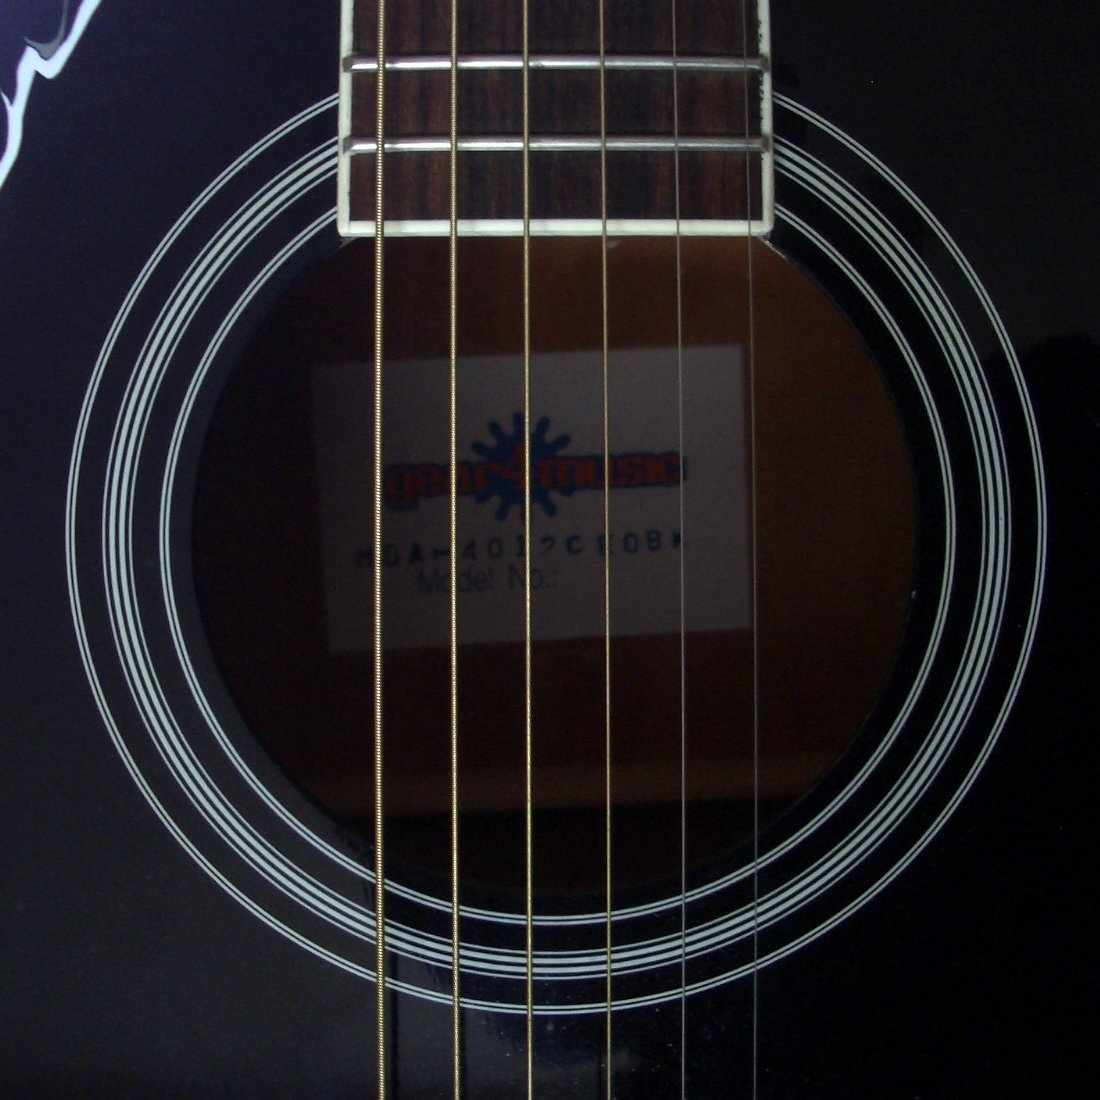
\includegraphics[width=0.95\textwidth]{circle.jpg}
  \begin{center}
    {\large ``Circle''}\par
    Foto di Howard Dickins\par
    \url{http://www.flickr.com/photos/dorkomatic/4551822855/}\par
    Licenza: Creative Commons Attribution 2.0\par
  \end{center}
\newpage

\section{Luoghi geometrici}

\begin{definizione}
Nel piano, si dice \emph{luogo geometrico} l'insieme di tutti e soli i punti del piano che verificano una proprietà, detta \emph{proprietà caratteristica} del luogo geometrico.
\end{definizione}
Ad esempio,
\begin{itemize*}
\item l'asse di un segmento è il luogo geometrico dei punti del piano equidistanti dagli estremi del segmento;
\item la bisettrice di un angolo è il luogo geometrico dei punti equidistanti dai lati dell'angolo.
\end{itemize*}
Se consideriamo la definizione ``costruttiva'' di asse di un segmento come retta perpendicolare al segmento stesso e passante per il suo punto medio, è possibile dimostrare che la nuova definizione di asse come luogo geometrico è ad essa equivalente.
Vale cioè il seguente
\begin{teorema}
Nel piano, il luogo geometrico dei punti equidistanti da due punti dati $A$ e $B$ è la retta $r$, perpendicolare al segmento $AB$ e passante per $M$, punto medio di $AB$.
\end{teorema}
Sia $r$ la retta perpendicolare ad $AB$ condotta da $M$, punto medio di $AB$. Dimostriamo che un generico punto $P\in r$ è equidistante da $A$ e $B$ e viceversa, un generico punto $Q$ tale che $QA\cong QB$ appartiene ad $r$.
~\\

\noindent Ipotesi: $r\perp AB$, $AM\cong MB$, $P\in r$.\tab Tesi: $PA\cong PB$.

\begin{proof}
Uniamo $P$ con $A$, $B$ ed $M$. Per ipotesi $PM \perp AB$, per cui, nel triangolo $PAB$, il segmento $PM$ è contemporaneamente altezza e mediana relative al lato $AB$; pertanto il triangolo $PAB$ è isoscele sulla base $AB$, da cui la tesi.
\end{proof}

\noindent Ipotesi: $QA\cong QB$.\tab Tesi: $Q\in r$.

\begin{proof}
Uniamo $Q$ con $A$, $B$ ed $M$. Per ipotesi il triangolo $QAB$ è isoscele sulla base $AB$; inoltre il segmento $QM$ è la mediana relativa alla base del triangolo isoscele, per cui $QM$ è anche altezza. dunque la retta $QM$ coincide con la retta $r$, cioè l'asse di $AB$.
\end{proof}

Analogamente, se consideriamo la classica definizione di bisettrice di un angolo come la semiretta interna all'angolo stesso avente origine nel suo vertice e tale da dividerlo in due angoli congruenti, possiamo dimostrare che la nuova definizione di bisettrice come luogo geometrico è equivalente a quest'ultima.
Vale cioè il seguente teorema.
\begin{teorema}
La bisettrice di un angolo è il luogo geometrico dei punti del piano equidistanti dai lati dell'angolo.
\end{teorema}
Sia $r\widehat{V}s$ un angolo (di vertice $V$ e di lati $r$ ed $s$) e sia $b$ la sua bisettrice (semiretta di origine $V$ che divide l'angolo a metà).
Verifichiamo prima che un generico punto $P\in b$ è equidistante da $r$ e da $s$.
~\\

\noindent Ipotesi: $P\in b$, $PK\perp s$, $PH\perp r$, $K\widehat{V}P\cong P\widehat{V}H$.\tab Tesi: $PK\cong PH$.

\begin{proof}
Tracciamo da $P$ le perpendicolari ai lati dell'angolo e chiamiamo $H\in r$ e $K\in s$ i piedi delle due perpendicolari. Osserviamo che i triangoli $VPH$ e $VPK$, rettangoli rispettivamente in $H$ e $K$, risultano congruenti perché hanno rispettivamente congruenti l'ipotenusa e un angolo acuto, per i criteri di congruenza sui triangoli rettangoli risultano congruenti. Pertanto i cateti $PH$ e $PK$, opposti a $V$, risultano congruenti, da cui la tesi ($P$ equidistante da $r$ e da $s$).
\end{proof}

Ovviamente, un qualsiasi punto appartenente ad una delle due semirette $r$ o $s$ che non sia il vertice $V$ non può essere equidistante da $r$ e da $s$, mentre il punto $V$ lo è (ha distanza nulla da entrambe).

Verifichiamo ora che, se $Q$ è un generico punto interno all'angolo $r\widehat{V}s$, se $Q$ è equidistante da $r$ e da $s$, deve risultare $Q\in b$.
~\\

\noindent Ipotesi: $PK\perp s$, $PH\perp r$, $PK\cong PH$.\tab Tesi: $K\widehat{V}P\cong P\widehat{V}H$.

\begin{proof}
Infatti, se tracciamo da $Q$ le perpendicolari alle semirette $r$ ed $s$ e chiamiamo $L\in r$ e $T\in s$ i piedi delle perpendicolari, per ipotesi risulta $QL\cong QT$. Se uniamo $Q$ con $V$, si vengono a formare due triangoli rettangoli $QLV$ e $QTV$ con l'ipotenusa $QV$ in comune ed una coppia di cateti congruenti. Tali triangoli risultano pertanto congruenti per il quarto criterio (più semplicemente per il criterio particolare dei triangoli rettangoli), e di conseguenza $L\widehat{V}Q\cong Q\widehat{V}T$, per cui la semiretta $VQ$ coincide con la bisettrice $b$.
\end{proof}


\section{Circonferenza e cerchio: definizioni e prime proprietà}

La definizione che ha dato Euclide di circonferenza fa riferimento ai luoghi geometrici: la circonferenza è il luogo geometrico dei punti del piano equidistanti da un punto del piano stesso, detto centro.
Intuitivamente, immaginiamo di fissare su di un piano un chiodo, di legare a questo chiodo una corda e di fissare all'altra estremità della corda una penna. Se facciamo ruotare la penna intorno al chiodo tenendo sempre in tensione la corda disegneremo una circonferenza.

\begin{definizione}
Assegnati nel piano un punto $C$ e un segmento $AB$, si chiama \emph{circonferenza} il luogo dei punti del piano che hanno distanza da $C$ congruente al segmento $AB$. Il punto $C$ viene detto centro della circonferenza, la distanza dei punti della circonferenza dal centro è detta \emph{raggio} della circonferenza.
\end{definizione}

\osservazione Una circonferenza divide il piano in 3 insiemi:
\begin{itemize*}
\item l'insieme dei punti la cui distanza dal centro è minore del raggio. Questi punti si dicono interni alla circonferenza.
\item l'insieme dei punti la cui distanza dal centro è uguale al raggio. Essi sono esattamente i punti della circonferenza.
\item l'insieme dei punti la cui distanza dal centro è maggiore del raggio. Questi punti si dicono esterni alla circonferenza.
\end{itemize*}

Se consideriamo l'unione dell'insieme dei punti della circonferenza con l'insieme dei punti interni alla circonferenza otteniamo un cerchio.

\begin{definizione}
Chiamiamo \emph{cerchio} la figura formata dai punti di una circonferenza e dai punti interni ad essa.
\end{definizione}

Abbiamo definito la circonferenza come un insieme di punti tutti equidistanti dal centro. Viceversa osserviamo che il centro è l’unico punto del piano equidistante da tutti i punti della circonferenza. Per questo motivo possiamo affermare che una circonferenza è individuata esattamente dal suo centro e dal suo raggio o equivalentemente dal centro e da un suo punto.

\begin{definizione}
Un segmento che ha come estremi due punti distinti di una circonferenza è detto \emph{corda}. In particolare, una corda che contiene il centro della circonferenza viene definita \emph{diametro}.
\end{definizione}

I punti estremi di un diametro vengono detti \emph{diametralmente opposti}.
Ogni diametro è il doppio di un raggio e tutti i diametri della stessa circonferenza sono fra essi congruenti. Il centro della circonferenza è anche il punto medio di ciascun diametro.
Diamo ora alcune importanti proprietà delle corde.

\begin{teorema}
Il diametro è la corda di lunghezza massima.
\end{teorema}

\begin{proof}
Data una circonferenza di centro $O$ e raggio $r$, consideriamo una corda qualsiasi $AB$. Se essa passa per il centro $O$, coincide con il diametro e dunque $AB=2r$; altrimenti essa può essere considerata come la base di un triangolo isoscele $AOB$ avente come lati i due raggi $OA$ e $OB$. In tal caso per la disuguaglianza triangolare un lato di un triangolo è minore della somma degli altri due lati e dunque possiamo scrivere: $AB < OA + OB$ ovvero $AB < 2r$.
In conclusione, il diametro è maggiore di qualunque altra corda che non passa per il centro.
\end{proof}

\begin{teorema}
L'asse di una corda qualsiasi passa per il centro della circonferenza.
\end{teorema}

\noindent Ipotesi: $A$ e $B$ due punti distinti appartenenti alla circonferenza, $a$ asse della corda $AB$.\tab Tesi: l'asse passa per il centro della circonferenza.

\begin{proof}
Congiungiamo $A$ e $B$ con il centro $O$ della circonferenza. Poiché $OA$ e $OB$ sono raggi della circonferenza, il triangolo $AOB$ è isoscele sulla base $AB$. Ricordiamo che l'asse relativo alla base di un triangolo isoscele contiene l'altezza (in figura $OH$).  Dunque $O$ appartiene all'asse $a$.
Se la corda $AB$ coincide con un diametro, $O$ ne è il punto medio; ma l'asse di un segmento è la retta perpendicolare al segmento nel suo punto medio, dunque anche in questo caso l'asse passa per il centro $O$ della circonferenza.
\end{proof}

\begin{teorema}
Un diametro passante per il punto medio di una corda è perpendicolare alla corda stessa.
\end{teorema}

\begin{proof}
In riferimento alla figura precedente e al teorema appena dimostrato, il diametro passa per ipotesi dal punto medio $H$ della corda $AB$ e per definizione da $O$, centro della circonferenza nonché vertice del triangolo isoscele $AOB$. Dunque $OH$ è mediana del triangolo $AOB$ relativamente alla base $AB$. Per il teorema sul triangolo isoscele, la mediana relativa alla base di un triangolo isoscele è anche altezza e quindi il diametro è perpendicolare alla corda $AB$.
\end{proof}

\begin{teorema}
In una circonferenza, corde congruenti hanno eguale distanza dal centro (e viceversa).
\end{teorema}

\noindent Ipotesi:
\begin{itemize*}
\item $AB\cong CD$ (corde congruenti),
\item $OH\perp AB$ ($OH$ distanza della corda $AB$ dal centro $O$),
\item $OK\perp CD$ ($OK$ distanza della corda $CD$ dal centro $O$).
\end{itemize*}
\noindent Tesi: $OH\cong OK$.

\begin{proof}
Consideriamo triangoli isosceli $AOB$ e $COD$; essi sono congruenti per il 3\textsuperscript{o} criterio di congruenza poiché per ipotesi le basi $AB$ e $CD$ sono congruenti e i lati $AO$, $OB$, $OC$ e $OD$ sono tutti raggi della circonferenza.
Di conseguenza anche le altezze $OH$ e $OK$ sono congruenti.
\end{proof}

Viceversa

\noindent Ipotesi:
\begin{itemize*}
\item $OH\cong OK$ (le distanze delle corde $AB$ e $CD$ dal centro $O$ sono congruenti),
\item $OH\perp AB$ ($OH$ distanza della corda $AB$ dal centro $O$),
\item $OK\perp CD$ ($OK$ distanza della corda $CD$ dal centro $O$).
\end{itemize*}
\noindent Tesi: $AB\cong CD$.

\begin{proof}
Consideriamo i triangoli rettangoli $AOH$ e $DOK$. $AO\cong DO\cong r$ (raggio della circonferenza) e $OH\cong OK$ per ipotesi; per il criterio particolare dei triangoli rettangoli, i due triangoli sono congruenti e quindi $AH\cong DH$. Allo stesso modo possiamo dimostrare che i triangoli rettangoli $BOH$ e $COK$ sono congruenti, per cui $BH\cong CK$. Dunque $AB \cong AH + BH \cong DK + CK \cong CD$.
\end{proof}

\begin{teorema}
Fra due corde diseguali, è maggiore quella che ha distanza minore dal centro (e viceversa).
\end{teorema}

\noindent Ipotesi:
\begin{itemize*}
\item $AB>CD$ (corde disuguali),
\item $OH\perp AB$ ($OH$ distanza della corda $AB$ dal centro $O$),
\item $OK\perp CD$ ($OK$ distanza della corda $CD$ dal centro $O$).
\end{itemize*}
\noindent Tesi: $OH\cong OK$.

\begin{proof}
A partire dal punto $A$ e allontanandosi dal punto $B$ si tracci la corda $AM$, consecutiva alla corda $AB$, in modo che $AM\cong CD$. Detta $OJ$ la distanza della corda $AM$ dal centro $O$, si ha che $OJ\perp AM$. Per il teorema precedente, essendo $CD$ e $AM$ corde congruenti, sarà $OJ\cong OK$; dunque basterà dimostrare che $OH < OJ$. Per ipotesi $AB > CD$, dunque $AB > AM$. Il senso di tale diseguaglianza vale anche per le rispettive metà dei segmenti $AB$ e $AM$, per cui $AH > AJ$ ($H$ è il punto medio di $AB$ e $J$ è il punto medio di $AM$ perché i triangoli $AOB$ e $AOM$ sono isosceli sulle basi $AB$ e $AM$, per cui $OH$ ed $OJ$, altezze relative alle basi, sono anche mediane).
Si congiunga $J$ con $H$ e si consideri il triangolo $HAJ$. A lato maggiore si oppone angolo maggiore (per le disuguaglianze tra gli elementi di un triangolo) per cui $H\widehat{J}A>A\widehat{H}J$; i rispettivi angoli complementari sono disuguali in verso opposto, quindi $H\widehat{J}O<O\widehat{H}J$. Relativamente al triangolo $HOJ$, poiché ad angolo minore si oppone lato minore (sempre per le disuguaglianze tra gli elementi di un triangolo, proprietà inversa della precedente), possiamo concludere che $OH < OJ$.
\end{proof}

Viceversa

\noindent Ipotesi:
\begin{itemize*}
\item $OH<OK$ (distanze disuguali),
\item $OH\perp AB$ ($OH$ distanza della corda $AB$ dal centro $O$),
\item $OK\perp CD$ ($OK$ distanza della corda $CD$ dal centro $O$).
\end{itemize*}
\noindent Tesi: $AB>CD$.

\begin{proof}
Utilizziamo un metodo simile alla dimostrazione per assurdo, come abbiamo già fatto per la dimostrazione delle disuguaglianze tra gli elementi di un triangolo: esaminiamo tutti i casi possibili ed escludiamo i casi che contraddicono il teorema precedente ed il primo caso di questo teorema.
Sono possibili le seguenti relazioni tra le lunghezze delle corde $AB$ e $CD$:
\[\text{(1) }AB\cong CD\text{;}\qquad\qquad\text{(2) }AB < CD\text{;}\qquad\qquad\text{(3) }AB > CD\text{.}\]

Se fosse vera la relazione (1), per il teorema precedente risulterebbe $OH\cong OK$, contro l'ipotesi.

Se fosse vera la (2), per la prima parte di questo stesso teorema risulterebbe $OH > OK$, contro l'ipotesi.

Rimane solo la possibilità che valga la relazione (3), la quale non è in contraddizione con la prima parte del teorema e che anzi la conferma. Dunque la tesi è verificata.
\end{proof}

Osservazioni:
\begin{itemize*}
\item Fissato un punto $P$, per esso passano infinite circonferenze.

Infatti basta considerare un qualunque altro punto $O$: quest'ultimo può essere il centro di una circonferenza di raggio $OP$.

\item Per due punti fissati $A$ e $B$ passano infinite circonferenze.

Infatti tutti i punti dell'asse del segmento $AB$ sono equidistanti da $A$ e da $B$ e dunque possono essere centri di circonferenze passanti per $A$ e per $B$.
\end{itemize*}

\begin{definizione}
L'insieme di tutte le circonferenze passanti per $A$ e per $B$ è detto \emph{fascio di circonferenze}. Chiamiamo $A$ e $B$ \emph{punti base del fascio}, la retta per $A$ e $B$ \emph{asse radicale} e \emph{asse centrale} l'asse del segmento $AB$ che contiene tutti i centri delle circonferenze del fascio.
\end{definizione}

\begin{teorema}
Per tre punti distinti non allineati passa una ed una sola circonferenza.
\end{teorema}

\begin{proof}
Siano $A$, $B$ e $C$ tre punti non allineati e congiungiamo $A$ con $B$ e $B$ con $C$. Allora gli assi dei segmenti $AB$ e $BC$ si intersecheranno in un punto $O$. Per la proprietà degli assi il punto $O$, appartenendo a entrambi gli assi, è equidistante dai punti $A$, $B$ e $C$. Allora si può costruire una circonferenza con centro in $O$ e raggio $OA$. Questa circonferenza passa per $A$, $B$ e $C$, inoltre è unica perché è unico l'asse di un segmento e di conseguenza è unico il punto di intersezione tra i due assi.
\end{proof}

\osservazione
L'ipotesi che i punti siano non allineati è essenziale. Seguendo le linee della dimostrazione, i segmenti $AB$ e $BC$ sono consecutivi ma non adiacenti, cosa essenziale per affermare che i rispettivi assi non sono paralleli. Vale infatti anche la seguente proprietà:
\begin{teorema}
Dati tre punti distinti $A$, $B$ e $C$ appartenenti ad una stessa retta, non esiste alcuna circonferenza che passa per $A$, $B$ e $C$.
\end{teorema}

\begin{proof}
Verifichiamo che non esiste alcun punto del piano individuato da $A$, $B$ e $C$ che possa essere il centro di una tale circonferenza, cioè che sia equidistante dai tre punti.
Supponendo per assurdo che esista un tal punto $O$, questo, dovendo essere equidistante da $A$ e da $B$, dovrebbe appartenere all'asse del segmento $AB$ (luogo dei punti equidistanti dagli estremi) e, per ragioni analoghe, dovrebbe appartenere anche all'asse del segmento $BC$. Ma i punti $A$, $B$ e $C$ sono distinti per ipotesi, in particolare $A$ e $C$ non sono sovrapposti. Quindi, detto $M$ il punto medio di $AB$ ed $N$ il punto medio di $BC$, $M$ ed $N$ sono anch'essi distinti e pertanto gli assi dei segmenti $AB$, $BC$ non possono essere coincidenti; inoltre gli assi dei segmenti $AB$, $BC$ sono entrambi perpendicolari alla stessa retta che contiene i tre punti $A$, $B$, $C$ e quindi sono paralleli tra loro; essendo dunque rette parallele e distinte, i due assi non hanno punti in comune e pertanto non può esistere un punto $O$ che possa essere il centro della circonferenza passante per $A$, $B$ e $C$.
\end{proof}

\begin{corollario}
Tre punti qualsiasi appartenenti ad una circonferenza non sono allineati.
\end{corollario}

A conclusione di queste prime proprietà, possiamo enunciare il seguente
\begin{corollario}
Una circonferenza è determinata univocamente dal suo centro e dal suo raggio oppure da tre suoi punti.
\end{corollario}

Diamo ora la definizione di alcune parti del cerchio e della circonferenza. Ne esamineremo le proprietà in seguito.
\begin{definizione}
Data una circonferenza di centro $O$,
\begin{itemize*}
\item chiamiamo \emph{angolo al centro} un qualunque angolo con vertice in $O$;
\item l'intersezione della circonferenza con un angolo al centro $\gamma$ è detta \emph{arco} e diremo che l'angolo $\gamma$ insiste su tale arco;
\item i punti di intersezione della circonferenza con i lati dell'angolo si dicono \emph{estremi dell'arco};
\item un arco individuato da un angolo al centro piatto si chiama \emph{semicirconferenza}.
\end{itemize*}
\end{definizione}

Ogni coppia di punti distinti su una circonferenza individua due archi sulla medesima circonferenza. Infatti se consideriamo $A$ e $B$ ottenuti come nella definizione precedente questi punti individuano l'arco su cui insiste l'angolo $\gamma$ ma anche la restante parte di circonferenza che è pure un arco.
Congiungendo $A$ con $B$ il segmento $AB$ è una corda della circonferenza. Diremo che la corda $AB$ sottende l'arco $AB$ o viceversa che l'arco insiste sulla corda.
Se in particolare i punti $A$ e $B$ sono diametralmente opposti, essi individuano sulla circonferenza due archi che sono due semicirconferenze.

\begin{definizione}Dato un cerchio
\begin{itemize*}
\item si dice \emph{settore circolare} l'intersezione del cerchio con un suo angolo al centro: se l'angolo al centro è piatto di parla di \emph{semicerchio};
\item si chiama \emph{segmento circolare ad una base} la parte di cerchio limitata da una corda e da un arco che vi insiste; la corda viene detta \emph{base del segmento circolare};
\item la parte di cerchio limitata da due corde parallele è detta \emph{segmento circolare a due basi}, le due corde prendono il nome di \emph{basi del segmento circolare} e la loro distanza si dice \emph{altezza del segmento circolare}.
\end{itemize*}
\end{definizione}

Ogni corda divide il cerchio in due segmenti circolari ad una base. In particolare se la corda è un diametro otteniamo due semicerchi.
Un semicerchio, quindi, è sia un particolare settore circolare sia un particolare segmento circolare. \`E anche l'unico caso possibile di settore che sia anche segmento o viceversa.

Una coppia di corde parallele individua in un cerchio un segmento circolare a due basi e due segmenti circolari ad una base (se vogliamo considerare solo le tre parti non sovrapposte che hanno in comune al massimo una corda). Più in generale, date due corde parallele e distinte, queste individuano un segmento circolare a due basi e quattro segmenti circolari ad una base, ed il segmento a due basi è anche l'intersezione dei due segmenti ad una base ``sovrapposti''.

\section{Posizioni relative fra rette e circonferenze}

Perché alcune strade a scorrimento veloce vengono chiamate ``tangenziali''?
Per rispondere a questa domanda dobbiamo definire le posizioni che può assumere una retta rispetto ad una circonferenza.
Consideriamo in uno stesso piano una circonferenza $C$ di centro $O$ e raggio $r$ e una retta generica $m$; la distanza $d$ fra il centro $O$ e la retta $m$ è definita dal segmento $OH$, che ha un estremo coincidente con il centro $O$ ed è perpendicolare in $H$ alla retta $m$ ($H$ è il piede della perpendicolare). Si possono distinguere i tre casi seguenti:

\begin{enumeratea}

\item $d > r$ : la distanza del centro $O$ dalla retta è maggiore del raggio.\\
Il punto $H$ è esterno alla circonferenza così come ogni altro punto della retta $m$. La retta si dice allora \emph{esterna} alla circonferenza e non ha alcun punto in comune con essa, ovvero non vi sono punti di intersezione fra $C$ ed $m$.

\item $d < r$ : la distanza del centro $O$ dalla retta è minore del raggio.\\
La retta $m$ interseca la circonferenza in due punti distinti $A$ e $B$; questi appartengono alla circonferenza e quindi $OA\cong OB\cong r$. Il segmento $AB$ appartiene alla retta e definisce anche la corda $AB$, i cui punti, tutti interni alla circonferenza, hanno una distanza dal centro minore del raggio; il punto di minore distanza è proprio $H$, che è anche il punto medio della corda $AB$. I punti della retta non appartenenti alla corda $AB$ sono esterni alla circonferenza e la loro distanza dal centro $O$ è maggiore del raggio.
La retta viene detta \emph{secante} alla circonferenza nei punti $A$ e $B$, che sono i punti di intersezione della retta con la circonferenza stessa.

\item $d = r$ : la distanza del centro $O$ dalla retta è pari al raggio.\\
Il punto $H$ appartiene alla circonferenza mentre ogni altro punto della retta $m$ è esterno alla circonferenza e ha una distanza dal centro $O$ maggiore del raggio. La retta viene detta \emph{tangente} alla circonferenza e $H$ è il punto di tangenza o di contatto.

\end{enumeratea}

Si noti che la retta tangente è perpendicolare al raggio nel punto di tangenza. Inoltre, l'unica retta perpendicolare al raggio nel punto di intersezione tra il raggio e la circonferenza è tangente.
Consideriamo una circonferenza $C$ di centro $O$ e raggio $r$ e una retta $m$ ad essa secante nei punti distinti $A$ e $B$. Sia $OH$ la distanza del centro $O$ dalla retta. 
Trasliamo la retta $m$ in modo da aumentare la sua distanza dal centro $O$ (vedi figura). All'aumentare della distanza $d = OH$, quella fra i punti $A$ e $B$ diminuisce; quando $OH = r$, i punti $A$ e $B$ coincidono nel punto di tangenza. Dunque la tangente è un caso particolare di secante avente due punti di intersezione coincidenti.

Una più efficace ``visualizzazione'' di questo concetto è la seguente.
Consideriamo la stessa circonferenza e la stessa retta dell'esempio precedente. Ruotiamo la retta attorno al punto $B$ (vedi figura).
La distanza del punto $A$ dal punto $B$ diminuisce all'aumentare dell'angolo $O\widehat{B}A$ fra la retta e il raggio. Quando il punto $A$ coincide con il punto $B$, il raggio è perpendicolare alla retta e quest'ultima è tangente alla circonferenza in $B\equiv A$.

Il lettore dimostri per esercizio il seguente teorema (si suggerisce di ricorrere alla dimostrazione per assurdo).
\begin{teorema}
Se una retta è esterna ad una circonferenza, allora la sua distanza dal centro è maggiore del raggio, se è tangente la distanza dal centro è uguale al raggio e se è secante la distanza dal centro è minore del raggio.
\end{teorema}

Possiamo ora rispondere al quesito iniziale. Il termine ``tangenziale'' viene utilizzato per descrivere una strada a scorrimento veloce, realizzata in zone particolarmente urbanizzate, per permettere il transito degli autoveicoli senza dover entrare in contatto diretto con la circolazione urbana; ciò comporta evidenti benefici per la vivibilità dei centri cittadini. Possiamo immaginare il centro città racchiuso in un cerchio e la tangenziale come una retta di un certo spessore che è, appunto, tangente al cerchio.

\begin{comment}

\subsection{Posizioni reciproche di due circonferenze}

Descriviamo adesso le posizioni reciproche di due circonferenze.
Due circonferenze si dicono:
1. esterne se tutti i punti dell'una sono esterni all'altra;
2. secanti quando hanno due punti in comune;
3. una interna all'altra se i loro raggi sono diseguali e i punti della circonferenza di raggio minore sono tutti interni a quella di raggio maggiore;
4. tangenti se hanno un solo punto in comune detto punto di tangenza; si può allora distinguere fra: 
   4a. tangenti esternamente, se ad eccezione del punto di tangenza, tutti i punti di una circonferenza sono esterni all'altra;
   4b. tangenti internamente, se i loro raggi sono diseguali e, ad eccezione del punto di tangenza, tutti  i punti della circonferenza di raggio minore sono interni a quella di raggio maggiore.

Analizziamo in dettaglio i diversi casi;  come esercizio lasciamo allo studente la dimostrazione rigorosa delle seguenti proprietà.



1. Quando le circonferenze sono esterne la distanza fra i due centri è maggiore della somma dei raggi.




Abbiamo già dimostrato che per tre punti distinti non allineati passa una sola circonferenza, mentre per due punti passano infinite circonferenze. Di conseguenza due circonferenze distinte possono avere al massimo due punti in comune. E' il caso delle circonferenze secanti. Se invece il numero di punti in comune è uno, allora ci riduciamo al caso delle circonferenze tangenti.
2. Quando due circonferenze si intersecano in due punti A e B, la distanza fra i centri è maggiore della differenza dei raggi e minore della loro somma.
La retta passante per i punti di intersezione viene detta asse radicale. 

Si dimostra che l’asse radicale è perpendicolare alla retta congiungente i centri.

3.Se una circonferenza è interna ad un'altra, e dunque ha raggio minore, la distanza fra i centri è minore della differenza fra i raggi.




Un caso particolare di circonferenze una interna all'altra è rappresentato dalle circonferenze concentriche, i cui centri coincidono. La zona di piano delimitata dalle due circonferenze è detta corona circolare.





4a. Quando due circonferenze sono tangenti esternamente in un punto T, la distanza fra i centri è uguale alla somma dei raggi. La retta tangente passante per T è comune alle due circonferenze ed è perpendicolare alla retta congiungente i due centri.







4b. Se le circonferenze sono tangenti internamente, la distanza fra i centri è pari alla differenza dei raggi.





Anche per le circonferenze si può affermare che sono tangenti in due punti coincidenti; infatti se prendiamo due circonferenze secanti e man mano allontaniamo i loro centri, osserviamo che i due punti di intersezione si avvicinano sempre più fino a sovrapporsi nel momento in cui la distanza fra i loro centri è pari alla somma dei raggi.

Se esaminiamo le varie posizioni reciproche nel caso di due circonferenze congruenti (r1 = r2 = r), tenendo conto anche del fatto banale che in questo caso | r1 - r2 | = 0 e r1 + r2 = 2r,  scompaiono le “distinte” possibilità che siano concentriche, interne, tangenti internamente, e compare la possibilità che siano coincidenti, cioè perfettamente sovrapposte.
Lasciamo al lettore la “rivisitazione” dei vari casi nell’ipotesi che le due circonferenze siano congruenti.

►4.  Angoli nelle circonferenze
Ricordiamo che abbiamo definito angolo al centro di una circonferenza di centro O e raggio r un qualsiasi angolo avente come vertice il centro O.
Tracciato un angolo al centro, i suoi lati intersecano la circonferenza in due punti P e Q e di conseguenza l’angolo contiene l’arco PQ; si dice che l’angolo al centro POQ insiste sull’arco PQ o sottende l’arco PQ.
Si noti che tracciate due semirette uscenti dal centro O, si vengono a formare due angoli al centro esplementari, ovvero la cui somma è un angolo giro, a cui corrispondono due distinti archi complementari PQ, la cui somma è il perimetro della circonferenza. 
I due angoli sono uno convesso e uno concavo, tranne il caso particolare in cui essi sono entrambi piatti, con le due semirette opposte. In tal caso, anche i relativi archi sono congruenti e ognuno ha misura pari al semiperimetro della circonferenza.
Diamo ora la seguente
DEFINIZIONE. Data una circonferenza di centro O e raggio r, si definisce angolo alla circonferenza qualsiasi angolo avente il vertice sulla circonferenza e i cui lati siano secanti o tangenti alla circonferenza stessa. 
In base alla definizione si possono distinguere tre casi:
i lati dell’angolo sono entrambi secanti alla circonferenza;
un lato è secante e l’altro tangente;
ambedue i lati sono tangenti.
Anche gli angoli alla circonferenza insistono su archi di circonferenza. Questi appartengono all’angolo stesso e sono delimitati dai punti di tangenza o di intersezione fra i lati dell’angolo e la circonferenza. Nella figura seguente gli angoli alla circonferenza e i rispettivi archi sono segnati in rosso. In verde i corrispondenti angoli al centro come segue dalla seguente definizione.

DEFINIZIONE. Un angolo al centro ed un angolo alla circonferenza si dicono corrispondenti se insistono sullo stesso arco.






TEOREMA. L’angolo alla circonferenza è la metà del corrispondente angolo al centro.
Ipotesi: α angolo alla circonferenza che insiste sull’arco PQ; β angolo al centro corrispondente.
Tesi:  β = 2α
Dimostrazione
Distinguiamo tre casi:

1) Un lato dell’angolo alla circonferenza passa per il centro e dunque si sovrappone al diametro.
Abbiamo due possibilità:

	1a) L’altro lato è secante alla circonferenza.
In riferimento alla figura a fianco, il triangolo OVQ è isoscele sulla base VQ, in quanto i lati OV e OQ sono due raggi della circonferenza; ne segue che gli angoli alla base sono congruenti e dunque . L’angolo al centro  giace sul prolungamento del lato OV e dunque  è un angolo esterno al triangolo OVQ. Per il teorema degli angoli esterni ad un triangolo, possiamo affermare che POQ è uguale alla somma degli angoli interni non adiacenti e quindi β = α + α = 2 α.

	1b) L’altro lato è tangente alla circonferenza.
In questo caso un lato coincide sempre con il diametro e l’altro è tangente alla circonferenza nel punto V = Q; poiché le rette tangenti alla circonferenza sono sempre ortogonali al raggio nel punto di tangenza, i due lati sono perpendicolari. Di conseguenza l’angolo α è un angolo retto e il corrispondente angolo al centro β è un angolo piatto, per cui β = 2 α.


2) Il centro O è interno all’angolo alla circonferenza
Anche in questo caso abbiamo due possibilità:
	2a) I lati dell’angolo alla circonferenza sono entrambi 	secanti.

Si conduca dal vertice V dell’angolo alla circonferenza  il diametro VT; si ottengono in tal modo due angoli alla circonferenza  la cui somma è proprio l’angolo . Tali angoli hanno il lato comune VT coincidente con il diametro e dunque, essendo  i rispettivi angoli al centro, possiamo applicare  ad ognuno di essi il risultato dimostrato al punto 1:  e .
Ma la somma degli angoli  è pari all’angolo al centro , corrispondente all’angolo alla circonferenza .
Dunque  .


	2b) Un lato dell’angolo alla circonferenza è tangente.

La dimostrazione è del tutto simile alla precedente. Il diametro VC divide l’angolo alla circonferenza  negli angoli . Per il primo angolo vale quanto già dimostrato al punto 1a e ribadito al punto precedente: detto  il corrispondente angolo al centro, possiamo scrivere. Inoltre,  è retto per costruzione, e difatti misura la metà del corrispondente angolo al centro , che è proprio un angolo piatto (vedi quanto dimostrato nel punto 1b). Anche in questo caso, essendo  l’angolo al centro corrispondente all’angolo , si dimostra che
.
Si noti che  è un angolo concavo, ovvero maggiore di un angolo piatto.


3) Il centro O è esterno all’angolo alla circonferenza
Anche qui abbiamo due casi:

	3a) Entrambi i lati dell’angolo alla circonferenza sono secanti.
Sia  l’angolo alla circonferenza. Tracciamo il diametro VT.  Per quanto dimostrato al punto 1a,  l’angolo al centro  è il doppio del corrispondente angolo alla circonferenza  è il doppio dell’angolo . Essendo  l’angolo al centro corrispondente all’angolo , possiamo  scrivere:



3b) Un lato dell’angolo alla circonferenza è tangente
La dimostrazione è analoga alla precedente e fa uso delle proprietà 1a e 1b. Tracciato il diametro VC ed essendo    gli angoli corrispondenti,  possiamo scrivere:











I seguenti corollari sono immediata conseguenza del precedente teorema.
COROLLARIO 1. Angoli alla circonferenza che insistono su uno stesso arco sono congruenti.
Infatti gli angoli alla circonferenza che nelle figura seguente insistono sull'arco PQ, misurano la metà dello stesso angolo al centro POQ.

COROLLARIO 2. Ogni angolo alla circonferenza che insiste su una semicirconferenza è retto.
Infatti il corrispondente angolo al centro è un angolo piatto.

Premesso che affinché  due circonferenze siano congruenti è sufficiente che abbiano lo steso raggio, sussistono i seguenti teoremi, di cui lasciamo la dimostrazione al lettore in quanto questa si effettua velocemente ricorrendo alla sovrapposizione tramite movimento rigido degli elementi di cui si vuole dimostrare la congruenza (in una stessa circonferenza questo si otterrà tramite rotazione intorno al centro).

TEOREMI
In una stessa circonferenza o in circonferenze congruenti, ad archi congruenti corrispondono angoli al centro e corde congruenti.
In una stessa circonferenza o in circonferenze congruenti, a corde congruenti corrispondono angoli al centro ed archi congruenti.
In una stessa circonferenza o in circonferenze congruenti, ad angoli al centro congruenti corrispondono archi e corde congruenti


►5.  Proprietà dei segmenti di tangenza
Data una circonferenza C di centro O e raggio r, ed un punto P del piano, quante sono le rette passanti per P e tangenti a C?  Ovviamente, dipende dalla posizione del punto P rispetto alla circonferenza C.  Se P è interno a C, non esiste alcuna retta passante per P e tangente a C, anche perché  OP < r.  Se invece il punto PC, allora esiste una ed una sola retta passante per P e tangente a C, ed in questo caso OP coincide con un raggio di C e la retta tangente è perpendicolare ad OP.

Se consideriamo un punto P esterno a C, allora esistono due rette distinte passanti per P e tangenti a C. Verifichiamo, con l’aiuto di una costruzione geometrica, che da un punto esterno ad una circonferenza possiamo tracciare due tangenti, e due sole, alla circonferenza stessa.
Uniamo P con O e costruiamo la circonferenza di diametro OP; le due circonferenze si intersecano in due punti distinti A, B. Uniamo A e B con O e con P. Gli angoli  sono retti perché sono angoli alla circonferenza che insistono su semicirconferenze. Dunque , per cui le rette AP e BP hanno distanza da O pari ad r, e quindi sono tangenti a C. A e B sono gli unici punti per cui valgono le relazioni precedenti, perché sono gli unici punti d’intersezione delle due circonferenze. AP e BP sono pertanto le due uniche rette passanti per P e tangenti a C.
I segmenti  AP  e  BP  che uniscono i punti di tangenza con il punto esterno P sono detti segmenti tangenti.

TEOREMA. I segmenti tangenti AP, BP condotti da un punto P ad una circonferenza sono congruenti.
Infatti, seguendo le linee della costruzione precedente, i triangoli rettangoli OPA e OPB hanno l’ipotenusa OP in comune e i cateti OA, OB congruenti perché raggi della stessa circonferenza; sono dunque congruenti per il criterio particolare dei triangoli rettangoli e di conseguenza gli altri due cateti AP, BP risultano congruenti, come volevasi dimostrare▄

Dalla congruenza dei due triangoli rettangoli segue anche la congruenza delle due coppie di angoli acuti:. Da queste due congruenze segue il seguente 
COROLLARIO. Il segmento OP che unisce il centro di una circonferenza con un punto esterno è bisettrice sia dell’angolo formato dalle due tangenti uscenti da P sia dell’angolo al centro avente come lati i raggi per i punti di tangenza.
Inoltre, OP è anche perpendicolare alla corda AB avente per estremi i punti di tangenza.
COROLLARIO. Date due circonferenze secanti, la congiungente dei loro centri è perpendicolare alla congiungente dei punti d’intersezione.
Lasciamo al lettore la dimostrazione del corollario.
Osservazioni 
La retta passante per i due punti d’intersezione di due circonferenze è detta asse radicale, e si parla di asse radicale in maniera più generale, cioè anche tra due circonferenze che tra loro non sono secanti. L’asse radicale non esiste solo nel caso in cui le due circonferenze siano concentriche. 
Nel caso in cui le due circonferenze siano tangenti (sia esternamente sia internamente), l’asse radicale coincide con la tangente in comune. 
Nel caso in cui le due circonferenze non abbiano punti in comune (o sono reciprocamente esterne, o sono l’una interna all’altra, ma non concentriche), l’asse radicale è una particolare retta esterna ad entrambe. 
L’asse radicale è perpendicolare alla congiungente dei centri ed è il luogo geometrico dei punti tali che, mandando da essi le tangenti alle due circonferenze risultano congruenti i quattro segmenti tangenti.
►6.  Poligoni inscritti e circoscritti ad una circonferenza

DEFINIZIONE. Un poligono si dice inscritto in una circonferenza se tutti i vertici del poligono appartengono alla circonferenza.

DEFINIZIONE. Un poligono si dice circoscritto a una circonferenza se tutti i suoi lati sono tangenti alla circonferenza.


TEOREMA. Se un poligono ha gli assi dei lati che passano per uno stesso punto allora il poligono può essere inscritto in una circonferenza, e viceversa se un poligono è inscritto in una circonferenza allora gli assi dei suoi lati si incontrano nel centro della circonferenza.
Dimostrazione a

Sia ABCDEF un poligono che ha gli assi dei suoi lati che passano per uno stesso punto O. Poiché O appartiene all’asse di AB e poiché l’asse è il luogo dei punti equidistanti dagli estremi, si ha che . Poiché O appartiene anche all’asse di BC allora O è equidistante dagli estremi di BC, cioè  . Poiché ciò vale per tutti i lati del poligono si ha: . Pertanto la circonferenza di centro O e raggio OA passa per tutti i vertici del poligono e il poligono risulta inscritto.

Dimostrazione b
Sia ABCDEF un poligono inscritto in una circonferenza e che ha quindi tutti i vertici sulla circonferenza, allora tutti i suoi lati sono corde della circonferenza, di conseguenza, per una proprietà delle corde, gli assi delle corde passano per il centro della circonferenza, e quindi tutti gli assi dei lati del poligono si incontrano nel centro della circonferenza.

TEOREMA. Se un poligono convesso ha le bisettrici degli angoli che passano tutte per uno stesso punto allora il poligono può essere circoscritto a una circonferenza, e viceversa se il poligono è circoscritto a una circonferenza allora tutte le bisettrici degli angoli del poligono passano per il centro della circonferenza.
Dimostrazione
ABCD sia il poligono convesso; AO la bisettrice dell’angolo in A e BO la bisettrice dell’angolo in B. Poiché la bisettrice è il luogo dei punti equidistanti dai lati dell’angolo si ha che il punto O è equidistante dal lato AD e dal lato AB, cioè . Analogamente, O, appartenendo alla bisettrice BO dell’angolo in B, è equidistante da AB e da BC, cioè . Ciò vale per tutti i lati del poligono, pertanto . Tracciando la circonferenza di centro O e raggio OH si ha la circonferenza inscritta al poligono.
La dimostrazione del teorema inverso si basa anch’essa sulla proprietà della bisettrice dell’angolo.

►7.  Punti notevoli di un triangolo
Circocentro
I vertici di un triangolo sono tre punti non allineati, dunque per essi passa una ed una sola circonferenza: il centro di tale circonferenza si trova come intersezione degli assi di due lati del triangolo. Il centro della circonferenza circoscritta al triangolo è appunto detto circocentro del triangolo.
TEOREMA. I tre assi dei lati di un triangolo si incontrano in uno stesso punto, detto circocentro.
Dimostrazione 
Sia ABC un triangolo e siano e l’asse di AB, d l’asse di BC, f l’asse di AC. Sia D il punto d’intersezione tra d ed e (che, come detto in precedenza, esiste perché le due rette, in quanto perpendicolari a due segmenti non paralleli, non possono essere parallele). Allora risulta   in quanto De, ed anche   in quanto Pd; dunque, per la proprietà transitiva della congruenza, risulta  , e quindi Pf. Pertanto D risulta equidistante dai tre vertici ed è quindi il centro della circonferenza circoscritta▄
Osservazione. 
Il circocentro di un triangolo può essere interno o esterno al triangolo o sul perimetro. Ricordando le proprietà degli angoli alla circonferenza, il circocentro è sul perimetro solo nel caso in cui il triangolo è rettangolo, ed in tal caso si trova sul punto medio dell’ipotenusa. 
Da ciò seguono le seguenti importanti proprietà: 
In un triangolo rettangolo, il punto medio dell’ipotenusa è equidistante dai tre vertici; 
In un triangolo rettangolo, la mediana relativa all’ipotenusa è congruente alla metà dell’ipotenusa stessa.
Sempre per le proprietà degli angoli alla circonferenza, il circocentro di un triangolo è interno al triangolo se il triangolo è acutangolo, mentre è esterno se il triangolo è ottusangolo (il corrispondente angolo al centro è rispettivamente convesso o concavo).
Incentro
Esiste uno ed un solo punto equidistante dai tre lati di un triangolo, pertanto un triangolo è sempre circoscrivibile ad una circonferenza, cioè esiste ed è unica la circonferenza inscritta in un triangolo.
TEOREMA. Le bisettrici dei tre angoli di un triangolo si incontrano in uno stesso punto, detto incentro.
Dimostrazione. Ricordiamo che la bisettrice è la semiretta che divide a metà l’angolo, essa è anche il luogo dei punti equidistanti dai lati dell’angolo. Consideriamo un triangolo ABC ed i suoi tre angoli interni. Poiché la somma dei angoli interni di un triangolo è un angolo piatto, abbiamo  e a maggior ragione , quindi poiché i lati AC e BC non sono paralleli a maggior ragione non possono essere parallele le bisettrici degli angoli interni di vertici A e B, anzi i segmenti di bisettrice sono certamente interni al triangolo. Detto D il punto d’intersezione delle bisettrici di  e di , verifichiamo che anche la bisettrice di  passa per D. Poiché D appartiene alla bisettrice di , è equidistante dai lati AB e AC (GD=DE); analogamente, poiché D appartiene alla bisettrice di , è equidistante dai lati AB e BC (GD=DF). Dunque Q deve essere equidistante dai lati AC e BC, pertanto, D deve appartenere alla bisettrice di . La distanza comune di D dai tre lati è il raggio della circonferenza inscritta nel triangolo, che ha centro D.

Ortocentro
Un altro punto notevole di un triangolo è il punto d’incontro delle altezze, detto ortocentro. Anche questo esiste ed è unico. Ricordiamo che di solito si parla di altezza come del segmento che unisce un vertice con il piede della perpendicolare al lato opposto. Qui ci occupiamo di retta dell’altezza, cioè della retta perpendicolare ad un lato di un triangolo e passante per il vertice opposto. Osserviamo infatti che, mentre l’incentro è certamente interno al triangolo, l’ortocentro può essere esterno al triangolo.
TEOREMA. Le tre altezze di un triangolo si incontrano in uno stesso punto, detto ortocentro.
Dimostrazione. Sia ABC un triangolo. Tracciamo la retta parallela a BC e passante per A; analogamente tracciamo la parallela ad AC passante per B e la parallela ad AB passante per C. Le tre rette, essendo parallele ai tre lati del triangolo ABC, sono a due a due incidenti. Chiamiamo A’ il punto d’intersezione tra AB ed AC, B’ il punto d’intersezione tra AB e BC, C’ il punto d’intersezione tra AC e BC.

Il triangolo BCA’ risulta congruente al triangolo ABC per il secondo criterio, in quanto ha BC in comune,  e  perché angoli alterni interni tra coppie di rette parallele tagliate dalla trasversale BC. Analogamente anche i triangoli ABC’ e ACB’ risultano congruenti ad ABC per il secondo criterio, quindi i quattro triangoli sono tutti congruenti. In particolare risulta che i segmenti C’A, AB’ e BC sono paralleli e congruenti, dunque la retta passante per A e perpendicolare a BC è sia l’altezza del triangolo ABC relativa al lato BC sia l’asse del segmento C’B’. Analogamente per le altre due altezze. Dunque le tre altezze del triangolo ABC coincidono con gli assi dei lati del triangolo A’B’C’: quindi l’ortocentro di ABC esiste perché coincide con il circocentro di A’B’C’.

Osservazione
Dalla costruzione precedente, risulta, pertanto ABC è acutangolo, rettangolo, ottusangolo come A’B’C’. Possiamo affermare dunque che:
se ABC è rettangolo, lo è pure A’B’C’, ed il punto medio dell’ipotenusa di A’B’C’ coincide con il vertice dell’angolo retto di ABC;
se ABC è ottusangolo, il suo circocentro è esterno ad esso, quindi l’ortocentro di ABC, dovendo essere esterno al triangolo A’B’C’, è a maggior ragione esterno ad ABC;
se ABC è acutangolo, quanto detto in precedenza ci permette solo di affermare che il circocentro di A’B’C’, che è anche l’ortocentro di ABC, è interno ad A’B’C’, ma in realtà è interno anche ad ABC.
Questo si vede meglio se consideriamo il classico modo di disegnare l’altezza: facciamo eventualmente compiere al triangolo una rototraslazione in modo che il lato rispetto a cui vogliamo tracciare l’altezza sia “orizzontale” ed il vertice opposto si trovi nel “semipiano in alto”; se il triangolo è acutangolo, comunque scegliamo il lato rispetto a cui vogliamo tracciare l’altezza, gli angoli compresi sono entrambi acuti, per cui il piede dell’altezza deve essere necessariamente interno al lato, e pertanto l’intera altezza (segmento) deve essere interna al triangolo. Come nel caso dell’incentro, che è sempre interno al triangolo, anche l’ortocentro è interno nel caso di triangolo ottusangolo. Lasciamo al lettore la dimostrazione dettagliata di queste due affermazioni (si può procedere per assurdo), ed illustriamo quanto detto nella figura seguente.
In riferimento alla figura del teorema precedente, l’ortocentro del triangolo ABC, e quindi anche il circocentro del triangolo A’B’C’, non può cadere all’interno di uno dei triangoli ABC’, AB’C, A’BC. 

Baricentro
Si chiama baricentro di un triangolo il punto d’incontro delle tre mediane. Poiché le mediane sono segmenti interni ad un triangolo, anche il baricentro lo è (segue banalmente dal teorema seguente che, oltre a dirci che il baricentro esiste ed è unico, ci dà anche un modo “operativo” per individuarlo).
TEOREMA DEL BARICENTRO. Le tre mediane di un triangolo si incontrano in un punto, detto baricentro, che divide ciascuna di esse in due parti tali che una (quella che contiene il vertice) è doppia dell’altra.
Dimostrazione
Si tratta di una delle principali conseguenze della corrispondenza di Talete, segue in particolare dal corollario riguardante i segmenti che uniscono i punti medi dei lati di un triangolo e dalle proprietà dei parallelogrammi. 
Dimostriamo prima che la tesi è verificata per il punto d’intersezione di due mediane, e poi dimostriamo che la terza mediana passa per quel punto.
Sia ABC un triangolo. Detti D, E, F i punti medi rispettivamente dei lati AC, BC, AB, tracciamo le mediane AE e BD. Queste, essendo interne al triangolo, certamente si incontreranno in un punto che chiamiamo G. Chiamiamo inoltre H il punto medio del segmento AG ed M il punto medio di BG. Uniamo D con E ed H con M. Nel triangolo ABC, DE è il segmento che unisce i punti medi dei lati AC e CB, dunque è parallelo al terzo lato AB ed è congruente alla sua metà. Ma nel triangolo ABG la stessa cosa vale per HM: è il segmento che unisce i punti medi dei lati AG e GB, per cui risulta parallelo al terzo lato AB e congruente alla sua metà. Pertanto i segmenti DE ed HM sono tra loro paralleli e congruenti. Questo ci consente di affermare che il quadrilatero HMED è un parallelogramma. Inoltre, per le proprietà dei parallelogrammi, le diagonali DM ed EH si dividono scambievolmente per metà, cioè il punto G è il punto medio sia di DM sia di EH. Dunque . Ma, per come abbiamo preso i punti H ed M, risulta anche  e  . Pertanto sono congruenti i segmenti AH, HG, GE (ognuno pari ad un terzo della mediana AE) ed anche tra loro congruenti i segmenti BM, MG, GD (ognuno pari ad un terzo della mediana BD). È dunque vero che BG misura il doppio di GD, come pure AG misura il doppio di GE.
Abbiamo dunque dimostrato che l’intersezione di due mediane è un punto interno al triangolo tale che divide ciascuna delle due mediane in parti che sono l’una il doppio dell’altra (quella che contiene il vertice è doppia dell’altra).
A questo punto, se il ragionamento fatto per le mediane AE e BD si ripete ad esempio per AE e CF, si può affermare che CF incontra AE in un punto tale che divide ciascuna delle due in due parti tali che quella che contiene il vertice è doppia dell’altra; ma tale punto su AE è già stato individuato: è il punto G. Quindi possiamo affermare che anche CF passa per il punto G ed inoltre il segmento CG è congruente al doppio del segmento GF. Questo conclude la dimostrazione del teorema del baricentro.

Excentri
Oltre ai principali punti notevoli di un triangolo esistono altri tre punti particolari, detti excentri, che sono i punti d’intersezione delle bisettrici degli angoli esterni. Illustriamo quanto affermato con una figura: i punti M, N, O sono gli excentri del triangolo ABC. Ricordando che la bisettrice è il luogo dei punti equidistanti dai lati di un angolo, notiamo ad esempio che il punto N, essendo l’intersezione delle bisettrici degli angoli esterni in B e C, è equidistante da BC e dai prolungamenti dei lati AC e AB: dunque è equidistante dalle rette dei tre lati del triangolo ABC. Se chiamiamo r la distanza di N da ciascuna delle rette dei tre lati di ABC, esiste una ed una sola circonferenza con centro N che ha come tangenti le rette dei tre lati, e tale circonferenza ha raggio r. Analogo discorso si può fare per gli altri due excentri, M ed O.

 
►8.  Proprietà dei quadrilateri inscritti e circoscritti
Per i quadrilateri, la proprietà di essere inscritto o circoscritto comporta notevoli proprietà. 
TEOREMA. Se un quadrilatero è inscritto ad una circonferenza, allora la somma di due angoli opposti è uguale alla somma degli altri due, ovvero un angolo piatto.
Dimostrazione
Aiutiamoci con il disegno a fianco. Consideriamo il quadrilatero ABCD inscritto nella circonferenza di centro O. Dimostriamo che la somma degli angoli in A e in C è un angolo piatto. Per fare questo, tracciamo gli angoli al centro insistenti sui due archi delimitati da D e B: i rispettivi angoli alla circonferenza saranno A e C. se chiamiamo  l’angolo in A, il relativo angolo al centro varrà  , per il teorema che lega angolo al centro e angolo alla circonferenza. Ripetiamo lo stesso procedimento per l’angolo in C, che chiamiamo : il relativo angolo al centro varrà . La somma degli angoli , ovvero l’angolo , forma un angolo giro, dunque la sua metà  è un angolo piatto. Ma  è proprio l’angolo in A, e  è quello in C. La loro somma, come volevamo dimostrare, dà un angolo piatto. Dato che la somma degli angoli interni di un quadrilatero è data da un angolo giro, sottraendo l’ampiezza degli angoli in A e in C, che insieme danno un angolo piatto, ottengo l’ampiezza della somma degli angoli in B e D, dunque, anche per questi ultimi due angoli, la somma è un angolo piatto▄

Si può dimostrare che vale anche il teorema inverso: se, in un quadrilatero, la somma degli angoli opposti è uguale a un angolo piatto, allora quel quadrilatero è inscrivibile ad una circonferenza.
Possiamo dunque enunciare il teorema completo.
TEOREMA INVERSO. Se un quadrilatero ha gli angoli opposti supplementari, allora il quadrilatero è inscrivibile in una circonferenza. 
Si dimostra per assurdo. Supponiamo che la circonferenza passi per ABC ma intersechi il quadrilatero in un punto P diverso da D. ABCP è quindi un quadrilatero inscritto in una circonferenza, e per il teorema diretto gli angoli opposti dovranno essere supplementari:, . Ma per ipotesi è anche , e quindi gli angoli  devono essere congruenti in quanto supplementari dello stesso angolo . Questo però è assurdo, in quanto avremmo che  , angolo esterno del triangolo ADP, sarebbe congruente ad un angolo interno non adiacente ad esso, mentre per il primo teorema dell’angolo esterno deve essere sempre maggiore di ciascuno dei due angoli interni non adiacenti ad esso. Dunque anche il punto D appartiene alla circonferenza▄




Vediamo ora alcune proprietà dei quadrilateri circoscritti
TEOREMA. Se un quadrilatero è circoscritto ad una circonferenza, allora la somma delle lunghezze di due suoi lati opposti è uguale alla somma delle lunghezze degli altri due.
Dimostrazione 
Sia il quadrilatero ABCD circoscritto alla circonferenza di centro O, come in figura. Siano P, Q, R, S i punti di tangenza rispettivamente dei lati AB, BC, CD, AD. Per il teorema sull’uguaglianza dei segmenti di tangente ad una circonferenza condotti da un punto esterno, si ha , , , , . Chiamando AP=p, BQ=q, CR=r, DS=s (vedi figura) si ha che:
AB+CD = AP+PB+CR+RD = p+q+r+s,
e che:
BC+AD = BQ+QC+DS+AS = p+q+r+s.
Per la proprietà transitiva dell’uguaglianza, ho che AB+CD=AD+BC, che è proprio quanto volevamo dimostrare.


TEOREMA INVERSO. Se in un quadrilatero la somma di due lati opposti è uguale alla somma degli altri due, allora il quadrilatero è circoscrivibile ad una circonferenza.
Anche questo teorema i dimostra per assurdo.
Supponiamo che il quadrilatero non sia circoscrivibile.
Sia ABCD il quadrilatero; tracciamo una circonferenza che sia tangente ai lati AB, BC e CD; questa esiste sicuramente poiché, se prolungassimo i lati AB (dalla parte di A) e CD (dalla parte di D), si formerebbe un triangolo, e in un triangolo è sempre possibile inscrivere una circonferenza. Supponiamo che la tangente condotta da A alla circonferenza intersechi la retta CD in un punto P diverso da D, che si trovi sul prolungamento del lato CD. Allora CP=CD+DP. Poichè ACBP è un quadrilatero circoscritto, possiamo applicare il teorema diretto: AP+BC=AB+CD+DP.
Per ipotesi abbiamo: AB+CD=AD+BC; sostituiamo nella relazione precedente AD+BC al posto di AB+CD; otteniamo: AP+BC=AD+BC+DP
Sottraendo ad ambo i membri BC si ottiene: AP=AD+DP. 
Siamo giunti all'assurdo, in quanto avremmo che nel triangolo ADP un lato è uguale alla somma degli altri due, mentre deve essere sempre minore. Quindi la tesi è vera.



►9.  Poligoni regolari
I poligoni regolari, cioè quelli che hanno tutti i lati e tutti gli angoli interni congruenti, sono sia inscrivibili sia circoscrivibili, e la circonferenza circoscritta e quella inscritta sono concentriche. 
Il centro comune alle due circonferenze si dice anche centro della figura. 
Nel caso di poligoni con un numero pari di lati, il centro coincide con il punto d’incontro di tutte le diagonali che congiungono vertici opposti. 
Nel caso di poligono con un numero dispari di lati, coincide con il punto d’incontro di tutti i segmenti che uniscono un vertice al punto medio del lato opposto.

TEOREMA. Se si divide la circonferenza in un numero n ≥ 3 di archi congruenti e si congiungono gli estremi di archi consecutivi, si ottiene un poligono regolare .
Dimostrazione
Dividiamo la circonferenza in 5 archi congruenti (vedi figura); otteniamo il pentagono ABCDE.
I lati del pentagono sono tutti congruenti, in quanto corde sottese da archi congruenti, ed anche gli angoli sono tutti congruenti, in quanto inscritti in archi congruenti (si ottengono infatti sommando due archi congruenti)
Dunque il pentagono è regolare poiché ha tutti i lati e tutti gli angoli congruenti.



TEOREMA. Se si divide la circonferenza in un numero n ≥ 3 di archi congruenti e si tracciano le tangenti alla circonferenza negli  estremi di archi consecutivi, i punti intersezione di tali tangenti sono i vertici di  un poligono regolare .
Dimostrazione
Dividiamo nuovamente la circonferenza in 5 archi congruenti, conduciamo le tangenti negli estremi degli archi; otteniamo il pentagono circoscritto ABCDE.
Congiungiamo ora gli estremi di tale archi, ottenendo, in base a quanto dimostrato prima, il pentagono regolare inscritto NOPQR. Consideriamo i triangoli che si vengono così a formare; sono tutti triangoli isosceli in quanto abbiamo: ;   in quanto angoli alla circonferenza che insistono sullo stesso arco; inoltre questi angoli sono tutti congruenti tra loro in quanto angoli alla circonferenza che insistono su archi congruenti. Infine i lati compresi tra questi angoli sono anch’essi tutti congruenti tra loro perché lati del pentagono regolare inscritto. Dunque questi triangoli sono tutti congruenti tra loro per il secondo criterio di congruenza. Da qui possiamo dedurre che  perché angoli al vertice di triangoli isosceli congruenti, e che  perché somme di segmenti congruenti (i lati obliqui dei triangoli isosceli). Quindi il poligono circoscritto, avendo tutti i lati e tutti gli angoli congruenti, è regolare.
TEOREMA. Ad ogni poligono regolare si può sempre circoscrivere una circonferenza ed in esso se ne può sempre inscrivere un’altra concentrica con la prima.
Dimostrazione
Consideriamo il pentagono regolare ABCDE. Tracciamo le bisettrici dei due angoli consecutivi , che s’incontrano in un punto O. Il triangolo BOA è isoscele poiché   in quanto metà di angoli congruenti, quindi sarà . Congiungiamo ora O con il vertice E. I triangoli BOA e AOE sono congruenti per il primo criterio di congruenza, poiché hanno : AO in comune, ABAE perché lati del poligono regolare,  perché metà dello stesso angolo. Dunque avremo che . Congiungendo successivamente O con gli altri vertici si arriva a dimostrare in modo analogo che: . Questo vuol dire che O è equidistante dai vertici del poligono,ed è quindi il centro della circonferenza circoscritta.
Dimostriamo ora che ABCDE è circoscritto ad un’altra circonferenza di centro O. I lati del poligono sono corde congruenti della circonferenza ad esso circoscritta, e sappiamo che corde congruenti hanno la stessa distanza dal centro. Dunque O è equidistante da tutti i lati del poligono, ed è perciò il centro della circonferenza inscritta. 
TEOREMA. Il lato dell’esagono regolare è congruente al raggio della circonferenza circoscritta.
Dimostrazione
Disegniamo la circonferenza circoscritta di centro O e raggio R, cosa che, in base al teorema precedente, è sempre possibile quando si tratta di un poligono regolare. Congiungiamo due vertici consecutivi dell’esagono con il centro della circonferenza e consideriamo il triangolo DOE. Questo triangolo è isoscele in quanto  perché raggi della circonferenza. Poiché se congiungessimo col centro O gli altri vertici del poligono otterremmo, per quanto dimostrato in precedenza,  sei triangoli congruenti, l’angolo al vertice  sarà di 60°, in quanto si ottiene dividendo per 6 l’angolo giro. Ma allora anche gli angoli alla base, essendo congruenti tra loro, saranno di 60°, e quindi il triangolo è equilatero, ed essendo , sarà anche . 


\newpage

% Copyright (c) 2015 Daniele Masini - d.masini.it@gmail.com

\section{Esercizi}

\subsection{Esercizi riepilogativi}

\begin{esercizio}
\label{ese:4.1}
Quali tra le seguenti sono proprietà del parallelogrammo?
\begin{enumeratea}
\item Ciascuna diagonale lo divide in due triangoli uguali\hfill\boxV\quad\boxF
\item Gli angoli opposti sono uguali\hfill\boxV\quad\boxF
\item Tutti i lati sono uguali\hfill\boxV\quad\boxF
\item Gli angoli sulla base sono uguali\hfill\boxV\quad\boxF
\item Le diagonali sono perpendicolari\hfill\boxV\quad\boxF
\item Gli angoli sono tutti congruenti\hfill\boxV\quad\boxF
\item Le diagonali sono anche bisettrici\hfill\boxV\quad\boxF
\end{enumeratea}
\end{esercizio}

\begin{esercizio}
\label{ese:4.2}
Vero o Falso?
\begin{enumeratea}
\item Un quadrilatero che ha i lati consecutivi a due a due congruenti è un deltoide\hfill\boxV\quad\boxF
\item Un quadrilatero che ha una sola coppia di lati opposti uguali è un trapezio\hfill\boxV\quad\boxF
\item Il trapezio scaleno ha tutti i lati diversi tra di loro per lunghezza\hfill\boxV\quad\boxF
\item Gli angoli adiacenti alla base maggiore di un trapezio rettangolo sono uno retto e uno acuto\hfill\boxV\quad\boxF
\item Un trapezio scaleno può avere due angoli opposti ottusi\hfill\boxV\quad\boxF
\item In un trapezio isoscele gli angoli adiacenti alla base minore sono ottusi\hfill\boxV\quad\boxF
\item In un trapezio isoscele sono congruenti le proiezioni dei lati obliqui sulla base maggiore\tab\hfill\boxV\quad\boxF
\item Le diagonali di un deltoide si incontrano nel loro punto medio comune\hfill\boxV\quad\boxF
\item Nel parallelogramma gli angoli adiacenti allo stesso lato sono supplementari\hfill\boxV\quad\boxF
\item Nel parallelogramma una delle due diagonali lo divide in due triangoli isosceli\tab\tab\tab\hfill\boxV\quad\boxF
\item Se le diagonali di un quadrilatero si dividono a metà allora è un parallelogramma\tab\tab\hfill\boxV\quad\boxF
\item Le diagonali del rombo sono anche bisettrici\hfill\boxV\quad\boxF
\item Se le diagonali di un parallelogramma sono uguali il parallelogramma è un quadrato\tab\tab\hfill\boxV\quad\boxF
\item Un parallelogramma che ha un angolo retto è un rettangolo\hfill\boxV\quad\boxF
\item Un parallelogramma che ha due lati consecutivi congruenti è un quadrato\hfill\boxV\quad\boxF
\item Un quadrilatero con due lati opposti congruenti è un trapezio\hfill\boxV\quad\boxF
\item Il rombo è anche un rettangolo\hfill\boxV\quad\boxF
\item Il rombo è anche quadrato\hfill\boxV\quad\boxF
\item Il rettangolo è anche parallelogrammo\hfill\boxV\quad\boxF
\item Il quadrato è anche rombo\hfill\boxV\quad\boxF
\item Il trapezio è anche parallelogrammo\hfill\boxV\quad\boxF
\item Alcuni rettangoli sono anche rombi\hfill\boxV\quad\boxF
\end{enumeratea}
\end{esercizio}

\begin{multicols}{2}

\subsubsection*{Dimostra le seguenti proprietà}

\begin{esercizio}
\label{ese:4.3}
Due parallelogrammi sono congruenti se hanno congruenti due lati consecutivi e l'angolo compreso.
\end{esercizio}

\begin{esercizio}
\label{ese:4.4}
Due rettangoli sono congruenti se hanno congruenti due lati consecutivi.
\end{esercizio}

\begin{esercizio}
\label{ese:4.5}
Due rombi sono congruenti se hanno congruenti le due diagonali.
\end{esercizio}

\begin{esercizio}
\label{ese:4.6}
Le diagonali di un trapezio isoscele si dividono in parti rispettivamente congruenti.
\end{esercizio}

\begin{esercizio}
\label{ese:4.7}
In un trapezio isoscele, la retta che congiunge i punti medi delle basi è perpendicolare alle basi stesse, ed interseca le rette dei lati obliqui nel loro punto d’intersezione.
\end{esercizio}

\begin{esercizio}
\label{ese:4.8}
Se un trapezio ha tre lati congruenti, le diagonali sono bisettrici degli angoli adiacenti alla base maggiore.
\end{esercizio}

\begin{esercizio}
\label{ese:4.9}
Dimostra che un rombo è diviso da una sua diagonale in due triangoli isosceli congruenti.
\end{esercizio}

\begin{esercizio}
\label{ese:4.10}
In un triangolo $ABC$ prolunga la mediana $AM$ di un segmento $MD$ congruente ad $AM$. Dimostra che il quadrilatero $ABCD$ è un parallelogramma.
\end{esercizio}

\begin{esercizio}
\label{ese:4.11}
Sia $ABCD$ un parallelogramma, siano $M$, $N$, $O$ e $P$ i punti medi dei lati. Dimostra che $MNOP$ è un parallelogramma.
\end{esercizio}

\begin{esercizio}
\label{ese:4.12}
Nel parallelogramma $ABCD$ prolunga di segmenti congruenti ciascun lato e sempre nello stesso senso. Dimostra che i nuovi vertici che si ottengono formano un parallelogramma.
\end{esercizio}

\begin{esercizio}
\label{ese:4.13}
Nel parallelogramma $ABCD$ si prendono sui lati opposti $AB$ e $CD$ i punti $E$ ed $F$ tali che $AE$ sia congruente a $CF$. Dimostra che anche $AECF$ è un parallelogramma.
\end{esercizio}

\begin{esercizio}
\label{ese:4.14}
Di un triangolo $ABC$ prolunga i lati $AB$ e $CB$ rispettivamente di due segmenti $BD$ e $BE$ tali che $AB\cong BD$ e $CB\cong BE$. Dimostra che $ACDE$ è un parallelogramma.
\end{esercizio}

\begin{esercizio}
\label{ese:4.15}
Unendo i punti medi di due lati opposti di un parallelogramma si ottengono due parallelogrammi.
\end{esercizio}

\begin{esercizio}
\label{ese:4.16}
Sulle diagonali $AC$ e $BD$ di un parallelogramma prendi i punti $A'$ e $C'$ su $AC$ in modo che $AA'\cong CC'$ su $BD$ prendi i punti $B'$ e $D'$ in modo che $BB'\cong DD'$. Dimostra che $A'B'C'D'$ è un parallelogramma.
\end{esercizio}

\begin{esercizio}
\label{ese:4.17}
Dato un parallelogramma $ABCD$ prolunga il lati nel seguente modo: $CD$ di un segmento $DE$, $DA$ di un segmento $DF$, $AB$ di un segmento $BG$, $BC$ di un segmento $CH$. Dimostra che se $DE\cong AF\cong BG\cong CH$ allora $EFGH$ è anche un parallelogramma.
\end{esercizio}

\begin{esercizio}
\label{ese:4.18}
Dato un segmento $AB$, sia $M$ il suo punto medio. Traccia rispettivamente da $A$ e da $B$ le rette $r$ ed $s$ parallele tra loro. Dal punto $M$ traccia una trasversale $t$ alle due rette che incontra $r$ in $C$ ed $s$ in $D$. Dimostra che $CADB$ è un parallelogramma.
\end{esercizio}

\begin{esercizio}
\label{ese:4.19}
Dimostra che in un parallelogramma $ABCD$ i due vertici opposti $A$ e $C$ sono equidistanti dalla diagonale $BD$.
\end{esercizio}

\begin{esercizio}
\label{ese:4.20}
Prolunga la mediana $AM$ di un triangolo isoscele di vertice $A$ di un segmento $MD$ congruente ad $AM$. Dimostra che $ABCD$ è un rombo.
\end{esercizio}

\begin{esercizio}
\label{ese:4.21}
Nel parallelogramma $ABCD$ sia $M$ il punto medio di $AB$ ed $N$ il punto medio di $DC$. Sia $P$ il punto di intersezione di $AN$ con $DM$ e $Q$ il punto di intersezione di $CM$ con $BN$. Dimostra che $PNAM$ è un rombo.
\end{esercizio}

\begin{esercizio}
\label{ese:4.22}
Dimostra che se un rombo ha le diagonali congruenti allora è un quadrato.
\end{esercizio}

\begin{esercizio}
\label{ese:4.23}
Dimostra che congiungendo i punti medi dei lati di un rettangolo si ottiene un rombo.
\end{esercizio}

\begin{esercizio}
\label{ese:4.24}
Dato un parallelogramma $ABCD$, siano $H$ e $K$ due punti della diagonale $AC$ in modo che $DH$ e $BK$ siano perpendicolari ad $AC$. Dimostra che $AH\cong KC$.
\end{esercizio}

\begin{esercizio}
\label{ese:4.25}
Sia $ABCD$ un trapezio di basi $BC$ e $AD$. Sia $r$ la bisettrice dell'angolo in $A$ ed $s$ la bisettrice dell'angolo in $B$. Dimostra che $r$ ed $s$ sono perpendicolari.
\end{esercizio}

\begin{esercizio}
\label{ese:4.26}
Nel parallelogramma $ABCD$ prolunga il lato $AB$ del segmento $AE$ e il lato $DC$ del segmento $CF$ congruente ad $AE$. Dimostra che anche $EBFD$ è un parallelogramma.
\end{esercizio}

\begin{esercizio}
\label{ese:4.27}
In un trapezio $ABCD$ la diagonale $AC$ è congruente alla base maggiore $AB$. Sia $M$ il punto medio del lato obliquo $BC$. Prolunga $AM$ di un segmento $ME$ congruente ad $AM$. Dimostra che $ABEC$ è un rombo.
\end{esercizio}

\begin{esercizio}
\label{ese:4.28}
Nel trapezio isoscele $ABCD$ con la base maggiore doppia della base minore, unisci il punto medio $M$ di $AB$ con gli estremi della base $DC$. Dimostra che $AMCD$ è un parallelogramma.
\end{esercizio}

\begin{esercizio}
\label{ese:4.29}
Nel trapezio isoscele $ABCD$ i punti $M$ e $N$ sono rispettivamente i punti medi delle basi $AB$ e $DC$. Dimostra che $MNCB$ è un trapezio rettangolo.
\end{esercizio}

\begin{esercizio}
\label{ese:4.30}
Siano $M$ e $N$ i punti medi dei lati obliqui di un trapezio isoscele $ABCD$. Dimostra che $BCMN$ è un trapezio isoscele.
\end{esercizio}

\begin{esercizio}
\label{ese:4.31}
Nel triangolo isoscele $ABC$ siano $BH$ e $BK$ le perpendicolari ai lati obliqui $AC$ e $AB$. Dimostra che $BCHK$ è un trapezio isoscele.
\end{esercizio}

\begin{esercizio}
\label{ese:4.32}
Dimostra che le proiezioni dei lati obliqui di un trapezio isoscele sulla base maggiore sono congruenti.
\end{esercizio}

\begin{esercizio}
\label{ese:4.33}
Nel triangolo isoscele $ABC$, di base $BC$, traccia le bisettrici agli angoli adiacenti alla base. Detti $D$ ed $E$ i punti di incontro di dette bisettrici rispettivamente con $AC$ e $AB$, dimostra che $EBCD$ è un trapezio isoscele.
\end{esercizio}

\begin{esercizio}
\label{ese:4.34}
Dimostra che in un trapezio isoscele che ha la base maggiore doppia della minore, le diagonali sono anche bisettrici degli angoli adiacenti alla base maggiore.
\end{esercizio}

\begin{esercizio}
\label{ese:4.35}
In un trapezio, il segmento che unisce i punti medi dei lati obliqui è parallelo alle basi e congruente alla loro semisomma.
\end{esercizio}

\begin{esercizio}
\label{ese:4.36}
Dato un qualsiasi quadrilatero $ABCD$, il quadrilatero non intrecciato avente come vertici i punti medi dei lati di $ABCD$ è un parallelogramma.
\end{esercizio}

\begin{esercizio}
\label{ese:4.37}
Il quadrilatero avente come vertici i punti medi dei lati di un trapezio isoscele è un rombo.
\end{esercizio}

\begin{esercizio}
\label{ese:4.38}
Dimostrare che, in un trapezio, il segmento che congiunge i punti medi dei lati non paralleli è uguale alla semisomma delle basi.
\end{esercizio}

\begin{esercizio}
\label{ese:4.39}
Dato un parallelogramma $ABCD$, si consideri il punto medio $M$ del lato $AB$, si congiunga il vertice $D$ con il punto $M$, si congiunga il vertice $A$ con il punto medio $N$ del segmento $DM$. Dimostrare che la retta $AN$ divide la diagonale $DB$ del parallelogramma in due parti di cui una è il doppio dell'altra.
\end{esercizio}

\begin{esercizio}
\label{ese:4.40}
Dato un triangolo qualunque $ABC$, si consideri il punto medio $M$ del lato $AB$, si consideri il segmento parallelo al lato $BC$ che parte da $M$ ed incontra il lato $AC$ nel punto $N$, si prolunghi questo segmento di un segmento $ND$ uguale ad $MN$. Dimostrare che il quadrilatero $MDCB$ è un parallelogramma.
\end{esercizio}

\begin{esercizio}
\label{ese:4.41}
Dato un quadrato $ABCD$ di centro $O$, siano $H$ e $K$ due punti sulla diagonale $AC$ simmetrici rispetto ad $O$. Dimostra che il quadrilatero $BHDK$ è un rombo. 
\end{esercizio}

\begin{esercizio}
\label{ese:4.42}
Dimostrare che un trapezio è isoscele se il punto medio della sua base maggiore è equidistante dagli estremi della base minore.
\end{esercizio}

\begin{esercizio}
\label{ese:4.43}
In un trapezio isoscele $ABCD$ (con base maggiore $AB$ e lati obliqui congruenti $BC$ e $AD$) sia $M$ il punto medio della base maggiore; prolungare $MC$ e $MD$ rispettivamente dei segmenti $CE$ e $DF$ fra loro congruenti. Dimostrare che il quadrilatero $ABEF$ è un trapezio isoscele.
\end{esercizio}

\begin{esercizio}
\label{ese:4.44}
Nel parallelogramma $ABCD$ si traccino da $A$ e da $C$ le perpendicolari alla diagonale $BD$; siano rispettivamente $E$ ed $F$ i punti di intersezione delle perpendicolari con la diagonale. Dimostra che $DE$ è congruente a $FB$ e che $AFCE$ è un parallelogramma.
\end{esercizio}

\begin{esercizio}
\label{ese:4.45}
Dato un parallelogramma $ABCD$, si consideri il punto medio $M$ del lato $AB$, si congiunga il vertice $D$ con il punto $M$, si congiunga il vertice $A$ con il punto medio $N$ del segmento $DM$. Dimostrare che la retta $AN$ divide la diagonale $DB$ del parallelogramma in due parti di cui una è il doppio dell'altra.	
\end{esercizio}

\begin{esercizio}
\label{ese:4.46}
Dato un triangolo qualunque $ABC$, si consideri il punto medio $M$ del lato $AB$, si consideri il segmento parallelo al lato $BC$ che parte da $M$ ed incontra il lato $AC$ nel punto $N$, si prolunghi questo segmento di un segmento $ND$ uguale ad $MN$. Dimostrare che il quadrilatero $MDCB$ è un parallelogramma.
\end{esercizio}

\begin{esercizio}
\label{ese:4.47}
Dato un quadrato $ABCD$ di centro $O$, siano $H$ e $K$ due punti sulla diagonale $AC$ simmetrici rispetto ad $O$. Dimostra che il quadrilatero $BHDK$ è un rombo.
\end{esercizio}

\begin{esercizio}
\label{ese:4.48}
Le diagonali di un trapezio isoscele dividono il trapezio in quattro triangoli, dei quali due triangoli sono isosceli e aventi gli angoli ordinatamente congruenti, mentre gli altri due triangoli sono congruenti.
\end{esercizio}

\begin{esercizio}
\label{ese:4.49}
Dimostra che il quadrilatero che si ottiene congiungendo i punti medi dei lati di un quadrilatero qualunque è un parallelogramma.
\end{esercizio}

\begin{esercizio}
\label{ese:4.50}
Che tipo di quadrilatero si ottiene congiungendo i punti medi dei lati di un rombo?
\end{esercizio}

\begin{esercizio}
\label{ese:4.51}
Che tipo di quadrilatero si ottiene congiungendo i punti medi dei lati di un rettangolo?
\end{esercizio}

\begin{esercizio}
\label{ese:4.52}
Dimostra che in un parallelogramma due vertici opposti sono equidistanti dalla diagonale avente per estremi gli altri due vertici.
\end{esercizio}

\begin{esercizio}
\label{ese:4.53}
In un parallelogramma $ABCD$ sia $M$ il punto medio di $AB$ e $N$ il punto medio di $DC$. Dimostra che $DMBN$ è un parallelogramma.
\end{esercizio}

\begin{esercizio}
\label{ese:4.54}
Dimostra che se in un parallelogramma le bisettrici di due angoli consecutivi si incontrano in un punto del lato opposto allora il parallelogramma ha un lato che è il doppio dell'altro.
\end{esercizio}

\begin{esercizio}
\label{ese:4.55}
Nel trapezio isoscele $ABCD$ le bisettrici degli angoli alla base maggiore $DC$ si incontrano in un punto $E$ sulla base minore. Dimostrare che $E$ è il punto medio della base minore.
\end{esercizio}

\begin{esercizio}
\label{ese:4.56}
Dimostra che un parallelogramma che ha tutte le altezze congruenti è un rombo.
\end{esercizio}

\begin{esercizio}
\label{ese:4.57}
In un trapezio le bisettrici degli angoli adiacenti alla base minore si intersecano in un punto della base maggiore. Dimostra che la base maggiore è congruente alla somma dei lati obliqui.
\end{esercizio}

\begin{esercizio}
\label{ese:4.58}
Disegna un trapezio isoscele con le diagonali perpendicolari. Dimostrare che il quadrilatero formato dai punti medi dei lati del trapezio è un quadrato.
\end{esercizio}

\begin{esercizio}
\label{ese:4.59}
Sia $AD$ bisettrice del triangolo $ABC$. Da $D$ traccia le parallele ai lati $AB$ e $AC$, detto $E$ il punto di intersezione del lato $AC$ con la parallela ad $AB$ ed $F$ il punto di intersezione del lato $AB$ con la parallela ad $AC$, dimostra che $AEDF$ è un rombo.
\end{esercizio}

\end{multicols}

\noindent\begin{minipage}{0.6\textwidth}\parindent15pt
\begin{esercizio}[Prove invalsi 2003]
\label{ese:4.60}
Il quadrilatero nella figura a fianco è simmetrico rispetto alla retta $AC$.
Sapendo che $B\widehat{A}C = 30\grado$ e $C\widehat{D}A = 70\grado$, quanto vale $B\widehat{C}D$?
\begin{enumeratea}
\item $140\grado$;
\item $150\grado$;
\item $160\grado$;
\item $165\grado$;
\item Le informazioni sono insufficienti.
\end{enumeratea}
\end{esercizio}
\end{minipage}\hfil
\begin{minipage}{0.4\textwidth}
	\centering% (c) 2014 Daniele Masini - d.masini.it@gmail.com
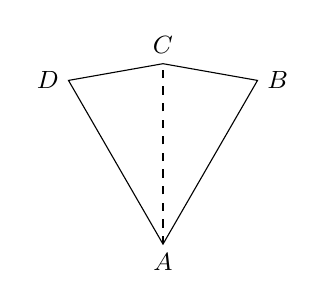
\begin{tikzpicture}[scale=1.2,font=\small]
\usetikzlibrary{calc, through, intersections}

\begin{scope}
\coordinate (a) at (0,0);
\coordinate (b) at (60:2);
\coordinate (d) at (120:2);
\coordinate (m) at ($(a)!.5!(b)$);

\path (b) -- +(170:1) coordinate (r2);
\coordinate (s2) at (90:1);
\coordinate (c) at (intersection of b--r2 and a--s2);
\draw[dashed] (a) -- (c);

\draw (a) node[below] {$A$} -- (b) node[right] {$B$} -- (c) node[above] {$C$} -- (d) node[left] {$D$} -- cycle;

\end{scope}

\end{tikzpicture}

\end{minipage}

\begin{esercizio}[Prove invalsi 2003]
\label{ese:4.61}
Quale fra le seguenti proprietà è falsa per tutti i parallelogrammi?
\begin{enumeratea}
\item I lati opposti sono uguali.
\item Gli angoli adiacenti sono supplementari.
\item Gli angoli opposti sono supplementari.
\item I lati opposti sono paralleli.
\item Le diagonali si dimezzano scambievolmente.
\end{enumeratea}
\end{esercizio}

\begin{esercizio}[Prove invalsi 2004]
\label{ese:4.62}
Quale tra le seguenti affermazioni riferite ad un parallelogramma qualsiasi è FALSA?
\begin{enumeratea}
\item I lati opposti sono paralleli.
\item Le diagonali sono uguali.
\item Gli angoli opposti sono uguali.
\item Ogni diagonale divide il parallelogramma in due triangoli uguali.
\end{enumeratea}
\end{esercizio}

\begin{esercizio}[Prove invalsi 2005]
\label{ese:4.63}
Quale tra le seguenti affermazioni relative ad un rombo è FALSA?
\begin{multicols}{2}
\begin{enumeratea}
\item Non ha i lati opposti paralleli.
\item Ha tutti i lati uguali.
\item Ha gli angoli opposti uguali.
\item Ha le diagonali perpendicolari.
\end{enumeratea}
\end{multicols}
\end{esercizio}

\begin{esercizio}[Prove invalsi 2005]
\label{ese:4.64}
Quale fra le seguenti condizioni è sufficiente affinché un quadrilatero sia un rettangolo?
\begin{enumeratea}
\item I lati opposti siano uguali e un angolo sia retto.
\item Le diagonali si dividano a metà.
\item I lati opposti siano paralleli.
\item Le diagonali siano uguali e un angolo sia retto.
\end{enumeratea}
\end{esercizio}

\begin{esercizio}[Prove invalsi 2006]
\label{ese:4.65}
Quale fra le seguenti affermazioni è vera?
Il quadrilatero avente i vertici nei punti medi dei lati di \ldots{}
\begin{enumeratea}
\item \ldots{} un rettangolo qualsiasi è sempre un quadrato.
\item \ldots{} un trapezio isoscele qualsiasi è un rettangolo.
\item \ldots{} un quadrilatero qualsiasi è un parallelogramma.
\item \ldots{} un quadrato è un rombo, ma non un quadrato.
\end{enumeratea}
\end{esercizio}

\begin{esercizio}[Prove invalsi 2007]
\label{ese:4.66}
Quale fra le seguenti affermazioni è falsa?
\begin{enumeratea}
\item Ogni rettangolo è anche un rombo.
\item Ogni rettangolo è anche un parallelogramma.
\item Ogni quadrato è anche un rombo.
\item Ogni rettangolo ha le diagonali uguali.
\end{enumeratea}
\end{esercizio}

\begin{esercizio}[Prove invalsi 2007]
\label{ese:4.67}
\`E dato un quadrilatero con le diagonali perpendicolari che si dimezzano scambievolmente.\\
Alberto afferma: <<Di sicuro si tratta di un quadrato.>>\\
Barbara afferma: <<Non è detto che sia un quadrato, ma di sicuro è un rombo.>>\\
Carla afferma: <<Non è detto che sia un quadrato, ma di sicuro è un rettangolo.>>\\
Daniele afferma: <<Si tratta certamente di un quadrilatero a forma di aquilone.>>\\
Chi ha ragione?
\begin{multicols}{4}
\begin{enumeratea}
\item Alberto;
\item Barbara;
\item Carla;
\item Daniele.
\end{enumeratea}
\end{multicols}
\end{esercizio}


\subsection{Risposte}

\begingroup
\hypersetup{linkcolor=black}

\paragraph{\ref{ese:4.1}.}
a)~V,\quad b)~V,\quad c)~F,\quad d)~F,\quad e)~F,\quad f)~F,\quad g)~F.

\paragraph{\ref{ese:4.2}.}
a)~F,\quad b)~F,\quad c)~V,\quad d)~V,\quad e)~F,\quad f)~V,\quad g)~V,\quad h)~F,\quad i)~V,\quad j)~F,\quad k)~F,\quad l)~V,\quad m)~F,\quad n)~V,\quad o)~V,\quad p)~F,\quad q)~F,\quad r)~F,\quad s)~V,\quad t)~V,\quad u)~F,\quad v)~V.

\paragraph{\ref{ese:4.60}.}
c.

\paragraph{\ref{ese:4.61}.}
c.

\paragraph{\ref{ese:4.62}.}
c.

\paragraph{\ref{ese:4.63}.}
a.

\paragraph{\ref{ese:4.64}.}
a.

\paragraph{\ref{ese:4.65}.}
c.

\paragraph{\ref{ese:4.66}.}
a.

\paragraph{\ref{ese:4.67}.}
b.

\endgroup


\cleardoublepage

\end{comment}
